%%%%%%%%%%%%%%%%%%%%%%%%%%%%%%%%%%%%%%%%%%%%%%%%%%%%%%%%%%%%%%%
%
% Welcome to Overleaf --- just edit your LaTeX on the left,
% and we'll compile it for you on the right. If you open the
% 'Share' menu, you can invite other users to edit at the same
% time. See www.overleaf.com/learn for more info. Enjoy!
%
%%%%%%%%%%%%%%%%%%%%%%%%%%%%%%%%%%%%%%%%%%%%%%%%%%%%%%%%%%%%%%%
\documentclass{beamer}
\usepackage[utf8]{inputenc}
\usepackage{minted} % Para sintaxe destacada de código
\usepackage{tikz}
%Information to be included in the title page:
\title{Acesso a reg's e wires (escopo)}
\author{Sophia Soares Mariano}
\institute{Poliware}
\date{2025}

\begin{document}

\frame{\titlepage}

\begin{frame}
\frametitle{Acesso a reg's e wires (escopo)}
Na linguagem Verilog, o escopo das variáveis define onde uma variável pode ser acessada ou utilizada dentro do código. As variáveis podem ser do tipo reg ou wire, cada uma com regras específicas de uso.
\end{frame}

\begin{frame}
\frametitle{Variáveis do tipo Reg}

As variáveis do tipo "reg" são usadas para armazenar valores que podem ser alterados ao longo do tempo, como em circuitos sequenciais. 
Elas podem ser acessadas dentro de blocos "always" e podem ser atribuídas valores dentro desses blocos. 
\end{frame}

\begin{frame}[fragile]{Exemplo: Uso de \texttt{reg} em Verilog}
\small
\begin{minted}[fontsize=\footnotesize, linenos]{verilog}
module exemplo_reg (
    input clk,
    input reset,
    output reg [7:0] saida // Variável do tipo reg
);

reg [7:0] contador; // Variável do tipo reg INTERNA

    always @(posedge clk or posedge reset) begin
        if (reset) begin
            saida <= 8'b0; // Atribuição não bloqueante
        end else begin
            saida <= saida + 1; // Incrementa a saída
        end
    end

    always @(*) begin
        contador = saida; // Acesso à variável reg dentro do always
    end

endmodule
\end{minted}
\end{frame}

\begin{frame}
\frametitle{Variáveis do tipo Reg}

Exemplo incorreto do uso de reg:
\begin{figure}
    \centering
    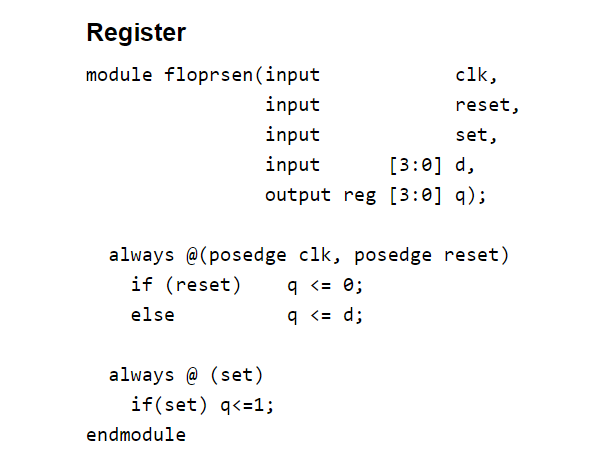
\includegraphics[width=0.5\linewidth]{reg.png}
    \caption{Exercício para encontrar o erro}
    Fonte: Chegg Inc.
    \label{fig:enter-label}
\end{figure}
\end{frame}

\begin{frame}
\frametitle{Variáveis do tipo Reg}
\begin{figure}
    \centering
    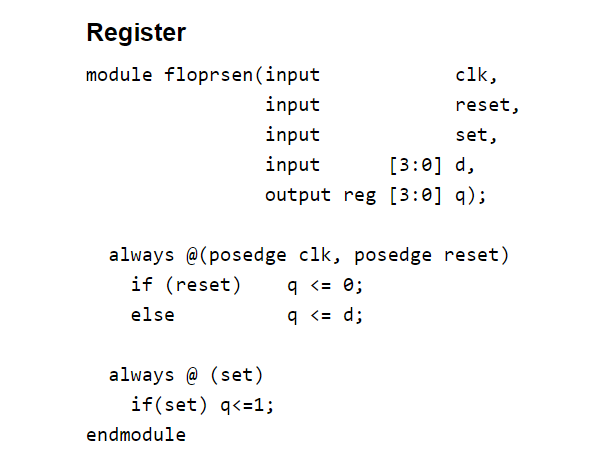
\includegraphics[width=0.5\linewidth]{reg.png}
    \label{fig:enter-label}
    \\
    Fonte: Chegg Inc.
\end{figure}

A variável q está sendo atribuída em dois blocos always diferentes, o que não é permitido para sinais do tipo reg em Verilog.
\end{frame}


\begin{frame}
\frametitle{Variáveis do tipo Wire}
As variáveis do tipo "wire" são usadas para conectar diferentes partes do circuito, como fios em um circuito físico.
Elas não podem armazenar valores, mas podem ser usadas para transmitir sinais entre módulos ou dentro de um módulo, em geral usando a operação "assign".
\end{frame}

\begin{frame}[fragile]{Exemplo: Uso de \texttt{wire} em Verilog}
\small
\begin{minted}[linenos]{verilog}
module exemplo_wire_assign (
    input  [7:0] a,
    input  [7:0] b,
    output wire [7:0] soma
);

    wire [7:0] resultado; // wire intermediário

    assign resultado = a + b; // Atribuição combinacional
    assign soma = resultado;  // Passa resultado para a saída

endmodule
\end{minted}
\end{frame}

\begin{frame}[fragile]{Exemplo: Uso incorreto de \texttt{wire} em Verilog}
\small
\begin{minted}[linenos]{verilog}
module exemplo_erro (
    input clk,
    input reset,
    output wire [7:0] saida
);

    wire [7:0] contador;

    always @(posedge clk or posedge reset) begin
        if (reset)
            contador <= 8'b0;
        else
            contador <= contador + 1;
    end

    assign saida = contador;

endmodule
\end{minted}
\end{frame}

\begin{frame}[fragile]{Exemplo: Uso incorreto de \texttt{wire} em Verilog}
\tiny
\begin{minted}[linenos]{verilog} 
module exemplo_erro (
    input clk,
    input reset,
    output wire [7:0] saida
);

    wire [7:0] contador;

    always @(posedge clk or posedge reset) begin
        if (reset)
            contador <= 8'b0;
        else
            contador <= contador + 1;
    end

    assign saida = contador;

endmodule
\end{minted}

\small
A variável contador foi declarada como wire, mas está sendo atribuída dentro de um bloco always, o que só é permitido para variáveis do tipo reg.
\end{frame}

\begin{frame}
\frametitle{Uso de ambas os tipos de variável em um único módulo}

Já que os usos desses dois tipos de dados são distintos e complementares, podem ser utilizados livremente, sem interferir um no outro.
\end{frame}

\begin{frame}[fragile]{Exemplo: Uso  de ambos os tipos de variável}
\tiny
\begin{minted}[linenos]{verilog}
module exemplo_reg_wire (
    input clk,
    input reset,
    output reg  [7:0] saida_reg,   // Saída do tipo reg
    output wire [7:0] saida_wire   // Saída do tipo wire
);

    // Variável interna do tipo reg (armazenamento)
    reg [7:0] contador;

    // Variável interna do tipo wire (valor combinacional)
    wire [7:0] dobro;

    // Lógica combinacional para calcular o dobro do contador
    assign dobro = contador << 1; // Equivalente a multiplicar por 2

    // Saída wire recebe o valor do dobro
    assign saida_wire = dobro;

    // Lógica sequencial: incrementa o contador a cada clock
    always @(posedge clk or posedge reset) begin
        if (reset) begin
            contador <= 8'd0;
            saida_reg <= 8'd0;
        end else begin
            contador <= contador + 1;
            saida_reg <= contador; // Armazena o valor do contador na saída reg
        end
    end

endmodule
\end{minted}
\end{frame}

\begin{frame}[plain]
    \centering
    {\Huge \textbf{Obrigado!}}
\end{frame}

\end{document}